\documentclass[conference]{IEEEtran}
\IEEEoverridecommandlockouts
% The preceding line is only needed to identify funding in the first footnote. If that is unneeded, please comment it out.
\usepackage{cite}
\usepackage{amsmath,amssymb,amsfonts}
\usepackage{algorithmic}
\usepackage{graphicx}
\usepackage{textcomp}
\usepackage{xcolor}

\ifCLASSOPTIONcompsoc
    \usepackage[caption=false, font=normalsize, labelfont=sf, textfont=sf]{subfig}
\else
\usepackage[caption=false, font=footnotesize]{subfig}

\def\BibTeX{{\rm B\kern-.05em{\sc i\kern-.025em b}\kern-.08em
    T\kern-.1667em\lower.7ex\hbox{E}\kern-.125emX}}
\begin{document}

\title{Control and data channel combining for reliability enhancement in Ultra-reliable and low-latency communication's downlink transmission\\
%{\footnotesize \textsuperscript{*}Note: Sub-titles are not captured in Xplore and
%should not be used}
%\thanks{Identify applicable funding agency here. If none, delete this.}
}

\author{\IEEEauthorblockN{Trung-Kien Le, Florian Kaltenberger}
\IEEEauthorblockA{\textit{EURECOM} \\
%\textit{name of organization (of Aff.)}\\
Biot, France \\
Emails: first name.last name@eurecom.fr}
\and
\IEEEauthorblockN{Umer Salim}
\IEEEauthorblockA{\textit{TCL Communication} \\
%\textit{name of organization (of Aff.)}\\
Paris, France \\
Emails: umer.salim@tcl.com}
%\and
%\IEEEauthorblockN{3\textsuperscript{rd} Given Name Surname}
%\IEEEauthorblockA{\textit{dept. name of organization (of Aff.)} \\
%\textit{name of organization (of Aff.)}\\
%City, Country \\
%email address}
%\and
%\IEEEauthorblockN{4\textsuperscript{th} Given Name Surname}
%\IEEEauthorblockA{\textit{dept. name of organization (of Aff.)} \\
%\textit{name of organization (of Aff.)}\\
%City, Country \\
%email address}
%\and
%\IEEEauthorblockN{5\textsuperscript{th} Given Name Surname}
%\IEEEauthorblockA{\textit{dept. name of organization (of Aff.)} \\
%\textit{name of organization (of Aff.)}\\
%City, Country \\
%email address}
%\and
%\IEEEauthorblockN{6\textsuperscript{th} Given Name Surname}
%\IEEEauthorblockA{\textit{dept. name of organization (of Aff.)} \\
%\textit{name of organization (of Aff.)}\\
%City, Country \\
%email address}
}

\maketitle

\begin{abstract}
5G will be supporting new services that have remarkably higher requirements than LTE 4G and Ultra-reliable and low-latency communication (URLLC) is one of those emerged categories. The strict requirements of URLLC demand new techniques in physical layer design. In this paper, we propose an intelligent combining of retransmissions of physical downlink control channel (PDCCH) and the physical downlink data channel (PDSCH). 
In the proposed scheme, the downlink control information (DCI) on PDCCH already indicates the location of a potential retransmission of the corresponding PDSCH and thus a retransmission of the DCI is only required when no HARQ feedback is received. Moreover, the retransmitted DCI can be combined with the first transmission so that resource consumption and latency are reduced compared to the conventional scheme. 
Theoretical calculations and simulation results show a decrease of latency and resource consumption as well as an increase of reliability in downlink transmission.  
\end{abstract}

\begin{IEEEkeywords}
5G, URLLC, PDCCH blocking, PDCCH combining, downlink scheduling scheme 
\end{IEEEkeywords}

\section{Introduction}
The advent of new paradigms like connected self-driving cars, automated industrial control, augmented and virtual reality led the wireless standardization bodies to take them into account. To that respect, 3GPP has defined three service categories for 5G: Enhanced Mobile Broadband (eMBB), Massive Machine-Type Communication (mMTC) and Ultra-Reliable Low Latency Communication (URLLC). 

Among these three service categories, URLLC raises the most challenge because it has to deal with two conflicting requirements: reliability and latency. Basically, one of two factors must be sacrificed to attain the other factor. To achieve a low latency, a shorter packet has to be used causing a degradation of reliability. In contrast, to raise the reliability, more resources are consumed due to parity check bits, retransmission and it is evident to increase latency.

\subsection{Techniques accepted in 3GPP Release 15}\label{IAA}
In Release 15, some modifications in frame structure of physical layer have been agreed to make the system compatible to new requirements. 

In LTE, subcarrier spacing (SCS) is fixed at 15kHz while in 5G, SCS can be selected flexibly among 30kHz, 60 kHz, 120kHz or even 240kHz \cite{ad2}. For this reason, the symbol length drops substantially and transmission latency is reduced.

Another option to reduce transmission latency is to do the transmission in mini-slot level instead of slot level \cite{ad3}. Therefore, the waiting time of an incoming packet falls rapidly.

Besides, in eMBB and URLLC multiplexing, pre-emption indication is used in downlink transmission \cite{ad4}. URLLC can be scheduled in the resource with an on-going eMBB transmission. The resource of eMBB overlapping that of URLLC is pre-empted and a preemption indication is transmitted to the UE in the same slot of eMBB transmission or the subsequent slots after the eMBB transmission. Based on this indication, the UE does not take the pre-empted part when decoding data.

\subsection{Techniques under research for next 3GPP releases}\label{IBB}
New techniques in transmission scheme to attain the latency and reliability requirements have attracted the attention of many companies. The proposals focus on repetition-based transmission aiming to relax the complexity of control and channel design. A repetition in frequency domain is proposed in \cite{b1}. The repetition of PDCCH in frequency domain is equivalent to a utility of a higher aggregation level (AL). It may cause PDCCH blocking due to a shortage of resources in a control resource set (CORESET) so the UEs have to wait for a CORESET in the next transmission occasion. Besides, a PDCCH repetition in time domain is considered in \cite{b2}. PDCCH can be repeated without waiting for hybrid automatic repeat request (HARQ) feedback and PDSCH is delayed until the success of PDCCH transmission. The process will stop when PDCCH is decoded successfully in the UE and the gNB receives ACK of PDCCH. After obtaining DCI from PDCCH, the UE can start to decode PDSCH. This method may cause a waste of resources if ACK feedback is not fast enough to stop the repetition process. In addition, it still might cause resource block in the next transmission occasion when an entire PDCCH is retransmitted.  

\cite{b3} considers a PDCCH repetition with asymmetric HARQ where the retransmission has a lower code rate than the initial transmission to increase reliability. Thanks to the retransmission, the requirement of block error rate (BLER) target for the initial transmission is relaxed and a high overhead to attain the low BLER target is eluded. Most of data is successful in the first transmission so the resource for the retransmission can be allocated to other UEs to avoid being wasted. However, in case the second transmission becomes necessary, it requires a much bigger resource than the first one that may lead to an increase of the blocking probability.

PDCCH feedback is proposed in \cite{b4} to speed up PDCCH repetition. A PDCCH feedback is transmitted from the UE to the gNB if PDCCH is decoded correctly. If PDCCH fails, there is no feedback to the gNB and it detects this discontinuous signal to trigger PDCCH repetition without waiting for HARQ feedback. Another proposal is to do back indication of PDSCH. This means that if the first PDCCH fails, this slot containing PDSCH is stored and back indicated by the second PDCCH. Thereby, the reliability is improved when two PDSCHs are combined together. However, the second transmission with both PDCCH and PDSCH might cause resource blocking that increases latency and decoding errors.

In \cite{b5}, in order to reduce the blocking probability and latency, PDCCH repetitions are generated by puncturing PDSCH of the eMBB UEs. This method increases the performance of PDCCH and decreases the blocking probability on the grounds that the repetitions are carried out in PDSCH region with more time and frequency resources than PDCCH region. Nevertheless, the performance of the eMBB UEs drops substantially due to the loss of the punctured bits\textquotesingle \, information.

In this work, a repetition-based downlink transmission scheme with a smart combining of PDCCHs and PDSCHs is described. Firstly, latency and reliability requirements of URLLC are analyzed in Section II. Section III is going to explain in detail the scheme and the techniques to implement it. Subsequently, standardization opportunity and challenges of the proposed scheme are discussed in Section IV. The simulation results are illustrated in Section V. Finally, Section VI provides a plan of future work and Section VII is the concluding remarks.

\section{URLLC requirements}
The requirement for URLLC is specified in \cite{b6}: ``A general URLLC reliability requirement for one transmission of a packet is 10\textsuperscript{-5} for 32 bytes with a user plane latency of 1ms''.

It is also noted in \cite{b6} that spectral efficiency and energy consumption also should be considered when trying to achieve a reliability target. 
\subsection{Analysis of URLLC latency}
Latency in physical layer can be expressed by the sum of 4 terms \cite{ad1}:
\begin{equation}
T\textsubscript{L}= T\textsubscript{ttt} + T\textsubscript{procTx} + T\textsubscript{prop} + T\textsubscript{procRx} + T\textsubscript{reTx},\label{eq1}
\end{equation}

\begin{itemize}
\item T\textsubscript{ttt}: time-to-transmit latency, is the time required to transmit a packet
\item T\textsubscript{prop}: propagation latency, is the time for a signal travel from the transmitter to the receiver
\item T\textsubscript{procTx}, T\textsubscript{procRx}: processing time for channel estimation, encoding and decoding of the first transmission
\item T\textsubscript{reTx}: time for the retransmission (containing T\textsubscript{ttt}, T\textsubscript{prop}, T\textsubscript{proc} and feedback time of the retransmission) 
\end{itemize}

In LTE, T\textsubscript{ttt} is fixed to 1ms while T\textsubscript{proc} and T\textsubscript{reTx} also contribute significantly to latency so URLLC latency requirement cannot be fulfilled. New frame structure and transmission scheme must be applied to URLLC to reduce latency as mentionned in in \ref{IAA} and \ref{IBB}.  
\subsection{Analysis of URLLC reliability}
In one-shot transmission, the error probability of a transmission is:
\begin{equation}
P^{e} = 1 - (1 - P^{e}_{c})(1 - P^{e}_{d}),\label{eq2}
\end{equation}

\begin{itemize}
    \item $P^{e}$ : the error probability of a transmission
    \item $P^{e}_{c}$ : the error probability of PDCCH 
    \item $P^{e}_{d}$ : the error probability of PDSCH
\end{itemize}

According to the URLLC requirement, the error probability is smaller than 10\textsuperscript{-5}. From \eqref{eq2}, in order to achieve that probability, it requires that the error probabilities of PDCCH and PDSCH are below 10\textsuperscript{-6}. The design of control and data channel to achieve this value is sophisticated and consumes remarkable time and frequency resources.

The complexity of channel design can be relaxed by considering a scheme with one retransmission in \cite{b7}. The successful probability of a transmission is:
\begin{equation}
P = P_{c}P_{d1} + (1-P_{c})P_{DTX}P_{c}P_{d1} + P_{c}(1-P_{d1})P_{N}P_{c}P_{d2},\label{eq3}
\end{equation}
\begin{itemize}
    \item $P_{c}$: the successful probability of PDCCH
    \item $P_{d1}$: the successful probability of a single PDSCH
    \item $P_{d2}$: the successful probability of a retransmitted PDSCH
    \item $P_{DTX}$: the successful probability of DTX or NAK detection if no ACK/NAK is sent by the UE
    \item $P_{N}$: the successful probability of DTX or NAK detection if NAK is sent by the UE
\end{itemize}

From \eqref{eq3}, the reliability of URLLC can be achieved with $P_{c}$, $P_{d1}$, $P_{d2}$, $P_{DTX}$ and $P_{N}$ being around 0.999. The requirements for control and data channel design are relaxed dramatically in comparison to a one-shot transmission. However, these values are still higher than the LTE probability of 0.99 and new techniques are necessary to enhance the performance of the channels so that the URLLC reliability target can be attained with a minimum number of retransmissions due to time constraint. This work focuses on increasing of $P_{c}$, $P_{d1}$ and $P_{d2}$ while $P_{DTX}$ and $P_{N}$ are assumed to be the same as LTE.

\section{PDCCH and PDSCH combining in downlink transmission of URLLC}

\subsection{Transmission scheme}\label{AA}
In the conventional transmission scheme with HARQ process, the gNB transmits PDCCH and PDSCH in the downlink at the beginning of the transmission. If the UE fails to decode PDCCH then PDSCH also cannot be decoded because its location is unknown to the UE so the gNB will not receive ACK/NACK from the UE. After detecting the missing HARQ response, the gNB knows that PDCCH is not detected by the UE. Thus, it reschedules data by sending again both PDCCH and PDSCH. It causes very sub-optimal resource usage because both control and data need to be transmitted again and most probably with lower code rate. Moreover, it leads to increase of data latency when the UE needs to wait for the retransmission. This latency can be a big issue for URLLC type of services. 

The retransmission of complete PDCCH and PDSCH as if it is a fresh transmission can be avoided by repeating PDCCH and PDSCH partially and combining these multiple transmitted PDCCHs and PDSCHs. In this scheme as shown in Fig.~\ref{fig1}, for the original transmission, the gNB transmits PDCCH (C1) and PDSCH (D1). When no HARQ response is received at the gNB for PDSCH at the expected time, it retransmits special versions of PDCCH and PDSCH that have shorter length in the next transmission occasion while the UE stores the current transmission occasion (containing C1 and D1). The two transmissions of control (C1 and C2) are designed such that they can be combined for joint detection (explained in \ref{BB}). Additionally to this, the combined PDCCH enables the UE to locate the two transmissions of PDSCH, the original transmission (D1) and the retransmission (D2) in order to combine them. This allows the network to enhance the reliability of both PDCCH and PDSCH for URLLC users in a very timely manner which can be a key to meet their latency and reliability requirements in harsh environments. 

\begin{figure}[htbp]
\centerline{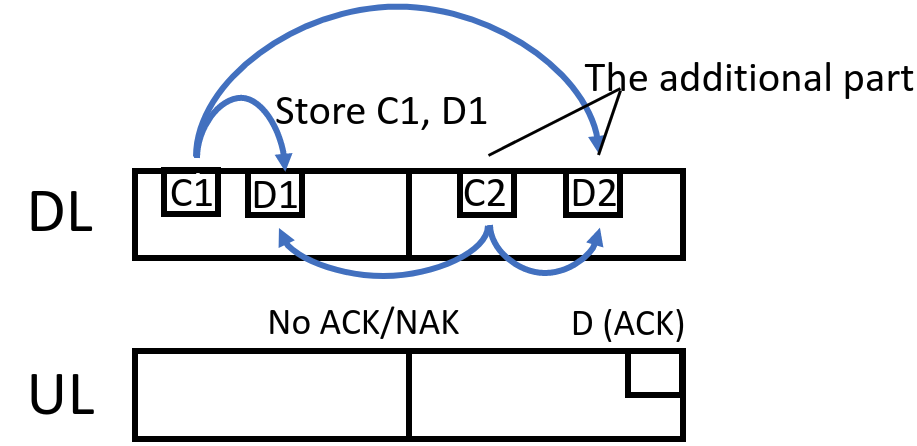
\includegraphics[scale=0.7]{fig1.png}}
\caption{Reliable transmission of DL assignment information.}
\label{fig1}
\end{figure}

To allow the combination of PDCCHs, the content of DCI on PDCCH must be the same for both the initial transmission and the retransmission. One way is to make the initial and retransmitted PDCCHs indicate the resource allocation information for both two transmissions as illustrated in Fig.~\ref{fig1}. This does not necessarily mean that all the fields in the DCI relevant to scheduling of resources, precoding, layers, MCS etc are doubled up. The resources for the retransmission PDSCH (D2) can be pre-defined as a function of resources indicated for the original transmission (D1). The other transmission parameters, like MCS, RV etc can remain the same.

In case the UE can decode PDCCH (C1) but encounters an error in decoding PDSCH (D1), PDSCH (D2) can be retransmitted independently in the next transmission occasion without a request of another PDCCH because the resource allocation information of this repetition is known by the UE by decoding the initial PDCCH. After that, the UE combines these two transmissions to decode data. It avoids the blockage of PDSCH repetition due to the shortage of resource for PDCCH. 

When the first DCI on PDCCH (C1) indicates locations of data transmissions on PDSCHs (D1 and D2) in the current slot and the next transmission slot, it means that the resource for the data retransmission is configured. It can lead to a waste of resources in case PDCCH and PDSCH are decoded successfully by the UE and there is no need for a retransmission. Therefore, this configured resource can be shared by a group of UEs and dynamically allocated to the UE needing a retransmission as shown in Fig.~\ref{fig2}. There is a need to retransmit data for the UE2 when it returns NACK while the other UEs return ACK. Therefore, the gNB retransmits data for the UE2 in D\textsubscript{rep}. The starting time of the initial transmissions is not required to be synchronized, the gNB only needs to receive HARQ feedback from the UEs before the starting time of the configured resource for the retransmission.

\begin{figure}[htbp]
\centerline{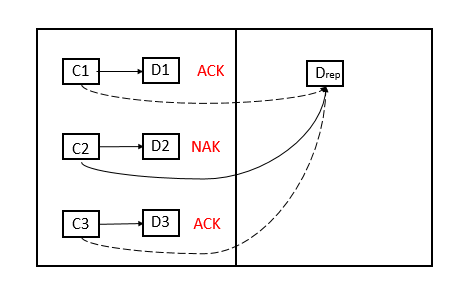
\includegraphics[scale=0.45]{fig2.png}}
\caption{Shared configured resource of PDSCH repetition.}
\label{fig2}
\end{figure}

The same principle can be applied to PDCCH repetition. A resource in the next transmission occasion is allocated to PDCCH repetition of a group of the UEs. If the first PDCCH is decoded and the retransmission is not necessary, the configured resource will be allocated to PDCCH of other UEs in the group.

One disadvantage of this method is that it only allows one UE with the first coming NACK an opportunity to receive a second transmission during D\textsubscript{rep}. Other UEs reporting a NACK are blocked from receiving a second transmission. However, due to a high reliability of URLLC transmission, the probability that two or more UEs encounter the errors at the same time is small (below 10\textsuperscript{-4}) so this method allows a good use of the configured resource. The blocking probability depends on the number of the UEs configured to that resource. Thus, the number of the UEs configured to a resource are chosen in order to balance the requirement of resource efficiency and reliability of URLLC.

\subsection{Design of PDCCH and PDSCH repetions}\label{BB}
\begin{figure}[htbp]
\centerline{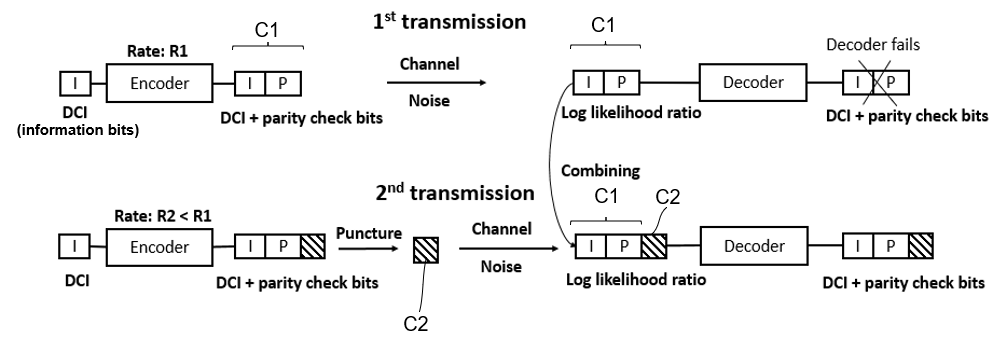
\includegraphics[scale=0.35]{fig3.png}}
\caption{Processing a DCI to form and combine two PDCCHs.}
\label{fig3}
\end{figure}

Fig.~\ref{fig3} shows in detail the contents of the multiple transmissions on PDCCH. When the transmission starts, the gNB encodes the control signal (DCI) using Polar code with the code rate R\textsubscript{1} to generate PDCCH containing DCI and parity check bits. PDCCH is transmitted from the gNB to the UE. The UE calculates the log likelihood ratios (LLRs) of the incoming codeword. The UE attempts to decode the incoming codeword and if the decoder fails to find the correct codeword, the UE stores the current slot containing PDCCH. This allows the UE to combine with PDCCH repetition in the next transmission occasion, in case the gNB retransmits the DCI. The buffered slot also comprises PDSCH. This allows the UE to retrieve the data on PDSCH if the PDCCH repetition is decoded successfully.

On the transmitter side, after not receiving ACK or NACK of the initial transmission from the UE, the gNB initiates the second transmission of DCI that has the same content with the first
DCI because both DCIs indicate the same PDSCHs. In this second transmission, a lower code rate R\textsubscript{2} (R\textsubscript{2} $<$ R\textsubscript{1}) is used in order to increase the reliability of PDCCH. There will be an overlap between the encoded bits at code rates R\textsubscript{1} and R\textsubscript{2}. The bits that have already been transmitted in the first transmission are punctured from the second transmission. This leaves only the additional bits due to the lower code rate are transmitted to the UE. The UE receives the second transmission and combines the additional bits (C2) with the stored bits (C1) of the first transmission in Fig.~\ref{fig3} to build a codeword with lower code rate R\textsubscript{2}. Due to the lower code rate, BLER for the combination ($P^{e}_{c}$ in \eqref{eq2}) is smaller than the BLER of the first transmission so the UE has a better chance to decode the transmitted DCI.

The content of DCI is the same for the initial transmission and the retransmission so the gNB generates a mother codeword of PDCCH with low rate. It selects suitable bits to be transmitted in the original PDCCH transmission and the repetition by applying puncturing. In this way, it does not need to encode PDCCH multiple times for multiple repetitions. 

The same principle is applied to PDSCH repetition to reduce resource consumption and increase reliability.

\subsection{Performance Analysis of the transmission scheme with PDCCH and PDSCH combining}\label{CC}

In the proposed scheme, only small parts of PDCCH and PDSCH are transmitted in the retransmissions. As a result, time for retransmission (T\textsubscript{reTx}) in \eqref{eq1} drops. The time margin gained might translate to a retransmission possibility in time constraint (1ms for URLLC) in case the channel is bad and PDCCH and PDSCH still fail to be correctly decoded after the first repetition. As shown in \eqref{eq2} and \eqref{eq3}, the reliability of control and data channel is relaxed when one repetition is allowed. The requirement of error probability drops from 10\textsuperscript{-6} in one-shot transmission to 10\textsuperscript{-3} in two-shot transmission (one initial transmission and one retransmission). Thereby, when the proposed scheme allows one more retransmission occasion, the reliability requirement of channel design can be relaxed further to reduce resource utilization. Otherwise, if the error probability is still kept to be 10\textsuperscript{-3} as in two-shot transmission, the reliability of the whole system is enhanced with one more retransmission if necessary. 

In addition, there is reduced blocking probability for the URLLC UEs as well as the eMBB UEs on the grounds that the gNB consumes less time and frequency resources for the retransmission proved by the following calculation. 

The length of DCI is $u$ (bits), the rates for the first and second transmissions are R\textsubscript{1} and R\textsubscript{2}, respectively. In the conventional HARQ process, the total number of the transmitted bits after 2 transmissions are $\frac{u}{R_{1}} + \frac{u}{R_{2}}$ (bits). While the number of the transmitted bits are only $\frac{u}{R_{2}}$ (bits) in the proposed scheme. Thereby, the number of the transmitted bits in PDCCH combining are 100 $\times$ $\frac{R_{1}}{R_{1} + R_{2}}$\% less than that of the conventional process. Let\textquotesingle s take an example with R\textsubscript{1} = $\frac{1}{3}$ and R\textsubscript{2} = $\frac{1}{6}$. This means that 33.33\% less bits are transmitted if PDCCH combining is applied.

According to \cite{b8}, the information bits of DCI format 0\_0 and DCI format 1\_0 are about 60 bits (depending on frequency and time assignments, modulation and coding scheme, etc) and CRC bits are 24 bits. In total, the payload size of DCI is about 84 bits. The rates of 2 transmissions are kept same as the above calculation: R\textsubscript{1} = $\frac{1}{3}$ and R\textsubscript{2} = $\frac{1}{6}$. When PDCCH combining is utilized, there are 252 bits saved. 1 resource element (RE) is allocated to 2 coded bits so 252 bits are equivalent to 126 REs being approximate to 12 physical resource blocks (PRBs) or 2 control channel elements (CCEs). With SCS being 30kHz, 1 PRB occupies a bandwidth of 30 kHz $\times$ 12 = 360 kHz. Thus, assuming 12 PRBs to be in 1 OFDM symbol, a bandwidth of 360 kHz $\times$ 12 = 4320 kHz = 4.3 MHz is spared and can be allocated to other UEs. 

The saving resource becomes significantly important when many UEs share resource together. For a PDCCH resource of 40 MHz and SCS of 30 kHz, there are maximum about 100 PRBs that are available to become PDCCH candidates in one symbol. The gNB can transmit 84 bits DCI with rate $\frac{1}{6}$ or $\frac{1}{12}$ to all UEs in the system that are equivalent to AL 4 or AL 8, respectively. A bandwidth of 40MHz with 100PRBs only can afford 2 UEs using AL 8. This means that if a PDCCH for UE1 is transmitted with AL 4 and fails to be decoded, a repetition is demanded. If a higher aggregation (AL 8) is utilized and the whole PDCCH repetition is transmitted, only 1 more PDCCH with AL 8 is able to be transmitted to another UE. Other UEs must wait until the next transmission occasion and it hampers the latency of the transmission. On the other hand, only AL 4 is required in the retransmission with PDCCH combining, 4 CCEs are spared for PDCCH of one more UE to transmit immediately in that occasion and it reduces latency due to resource block.

\subsection{Containing the complexity of blind decode for PDCCH combining}\label{DD}

The scheme in \ref{AA} and \ref{BB} requires the UE to combine multiple PDCCHs from different control occasions. This presents a challenge to UE blind decoding complexity if no additional constraints on PDCCH mapping are enforced. In principle, the location of PDCCH is unknown to a UE so each UE must perform blind decode until it finds a DCI that passes the CRC. When a UE is not able to decode a DCI on PDCCH, the UE is not certain if it failed to decode a DCI or if there was no DCI intended for that UE. 

In the PDCCH combining, the complexity of blind decode becomes more severe when the number of blind decodes grows remarkably. The UE monitors the current control resource to determine by blind decoding if a new DCI for the UE is received in the slot. If the UE fails to detect a PDCCH intended for it, it combines the current monitored occasion with the previous stored occasion for a potential combining. The number of stored occasion is limited to 1 to reduce memory and energy consumption. Fig.~\ref{fig4}\subref{4a} shows this results in a large number of blind decode combinations of the different PDCCH candidates. In a fully exhaustive scheme, the maximum number of combinations is the product of PDCCH candidates in two control occasion. 

\begin{figure}[htbp]
\centering
\subfloat[No mapping.\label{4a}]{%
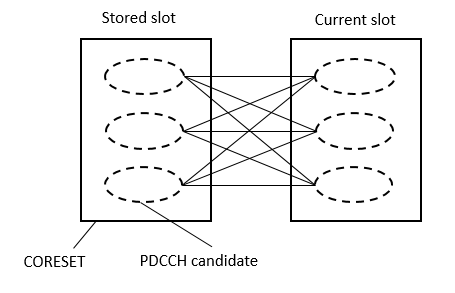
\includegraphics[scale=0.32]{fig4.png}}
\hfill
\qquad
\subfloat[One-to-one mapping.\label{4b}]{%
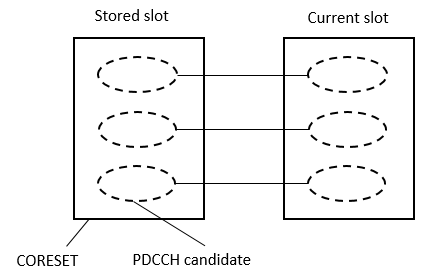
\includegraphics[scale=0.32]{fig5.png}}
\hfill

\caption{Combining of blind decode candidates.}
\label{fig4}
\end{figure}

The number of blind decodes in PDCCH combining decreases dramatically if the gNB is configured to transmit PDCCH and the repetition in the candidates with a one-to-one correspondence mapping. Fig.~\ref{fig4}\subref{4b} shows an example scheme where the UE only needs to attempt to combine the first PDCCH candidate in the current slot with the first PDCCH candidate in the stored slot. The process continues similarly with the second and third PDCCH candidates.The total number of combinations is significantly lower than that of Fig.~\ref{fig4}\subref{4a}. Other mapping possibilities are possible. The mapping rules may be defined a-priori in standards specifications or may be configured between the gNB and the UE. 

Based on the same principle of one-to-one correspondence of PDCCH
combining, the improvement of URLLC\textquotesingle s service quality through interference cancellation and frequency diversity in PDCCH transmission can be achieved by frequency hopping. In one
method, PDCCH candidates can be in different CORESETs in the same band but these candidates are hopped over different frequencies. The mapping is defined in such a manner so as to exploit the frequency diversity as much as possible within the resources configured for the CORESET. To contain the number of frequency hopping possibilities and eventual blind decode burden, there is an association between locations in the two occasions, such as a one-to-one correspondence between the candidates where PDCCH hops as illustrated in Fig.~\ref{fig5}\subref{5a}.

In another method to allow additional frequency diversity advantage in PDCCH combining, the initial transmission and repetition are allocated to the disjoint frequency bands with large frequency distance. As NR does not allow a single CORESET to change its frequency allocation in time, one way to achieve this is that the gNB configures two CORESETs at disjoint frequency locations as illustrated in Fig.~\ref{fig5}\subref{5b}. The rules to map between the PDCCH candidates of the two CORESETs can be defined in the same way as described earlier to contain the blind decode complexity. 

\begin{figure}[htbp]
\centering
\subfloat[Same band's CORESETs.\label{5a}]{%

\includegraphics[scale=0.33]{fig6.png}}
\hfill
\qquad
\subfloat[Different bands' CORESETs.\label{5b}]{%

\includegraphics[width=40mm,height=30mm]{fig7.png}}
\hfill
\caption{Frequency hopping in PDCCH combining.}
\label{fig5}
\end{figure}
\section{Standardization opportunity and challenges}

In LTE, soft combining of PDSCHs with different redundancy versions has been standardized and used. For this reason, a transmission scheme with a smart combining of PDCCHs also has good opportunity to be standardized in 5G NR. The idea takes advantage of the standardized scheme in HARQ process and improves it further to achieve the new strict requirements of 5G NR, especially URLLC.

There still exists the challenges and some prerequisites that need to be standardized in the next 3GPP releases to make the implementation of this scheme feasible. The mapping rule plays a pivotal role in PDCCH combining to reduce the number of blind decodes. However, it also reduces the scheduling flexibility of the gNB so it is necessary that 3GPP considers the advantages and disadvantages of mapping rule in different scenarios so as to accept and make it become standard. In addition, memory and power consumption of the UE must be enhanced. The reason is that a UE must always find and decode the incoming DCI in two steps. First, it decodes the current slot to check the presence of PDCCH. Subsequently, if no PDCCH is found, the UE combines the current slot with the previous slot to increase reliability of PDCCH so it has more chance to decode correctly PDCCH if it exists. Then if there is no PDCCH found, that slot is stored for the combining of next transmission occasion so memory of the UE has to be taken into account. A specification must be agreed among the manufacturers to guarantee the ability of the UE devices to be compatible with the proposed scheme. The next point is to define the fields of DCI because one DCI is used to indicate resource allocation of two PDSCHs.  

\section{Simulation results}

The simulation is performed in link level. Polar code is used to encode the input codeword (DCI) with 48 bits consisting of 24 information bits and 24 CRC bits. The encoding mechanism of the encoder follows 3GPP standard \cite{b8}. The code rate is 0.3 for the first transmission and 0.2 for the second transmission. The output codeword is modulated in QPSK and transmitted in channel. The decoder calculates LLRs and uses them to decode the receiving signal. The decoder is min-sum Successive cancellation list (SCL) decoder with list size 8 \cite{b9}.

\begin{figure}[htbp]
\centerline{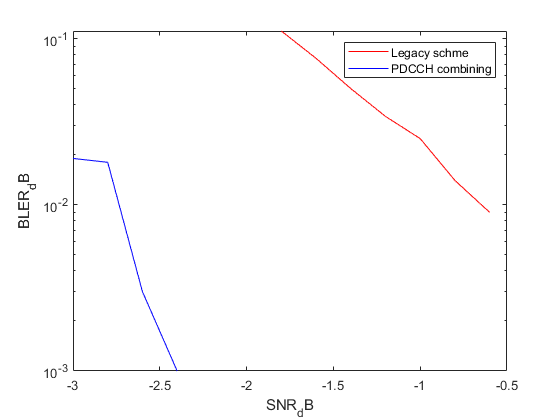
\includegraphics[scale=0.43]{fig8.png}}
\caption{BLER of PDCCH combining.}
\label{fig8}
\end{figure}

Fig.~\ref{fig8} shows BLER of PDCCH combining in comparison to the legacy NR scheme. In the first transmission, the output codeword on PDCCH with code rate 0.3 has 160 bits and is transmitted to the receiver. In the second transmission, a lower code rate 0.2 is used to generate a longer output codeword corresponding to 240 bits but only the additional bits due to a lower code rate are transmitted. For this reason, only 80 bits instead of 240 bits are transmitted in the second transmission. At the decoder, the LLRs of the first transmission and the second transmission are combined and the decoder decodes the codeword with the rate 0.2. The performance of the combined codeword represented by the blue curve is remarkably better than that of the transmission as in the legacy NR scheme represented by the red curve with a margin being about 2dB. This means that the information of the additional bits in the second transmission increases the reliability of PDCCH transmission without consuming much resources for the second transmission of the whole PDCCH with a higher AL as in the conventional scheme as shown in \ref{CC}. When $P^{e}_{c}$ in \eqref{eq2} decreases, the whole transmission's reliability increases.  

\begin{figure}[htbp]
\centerline{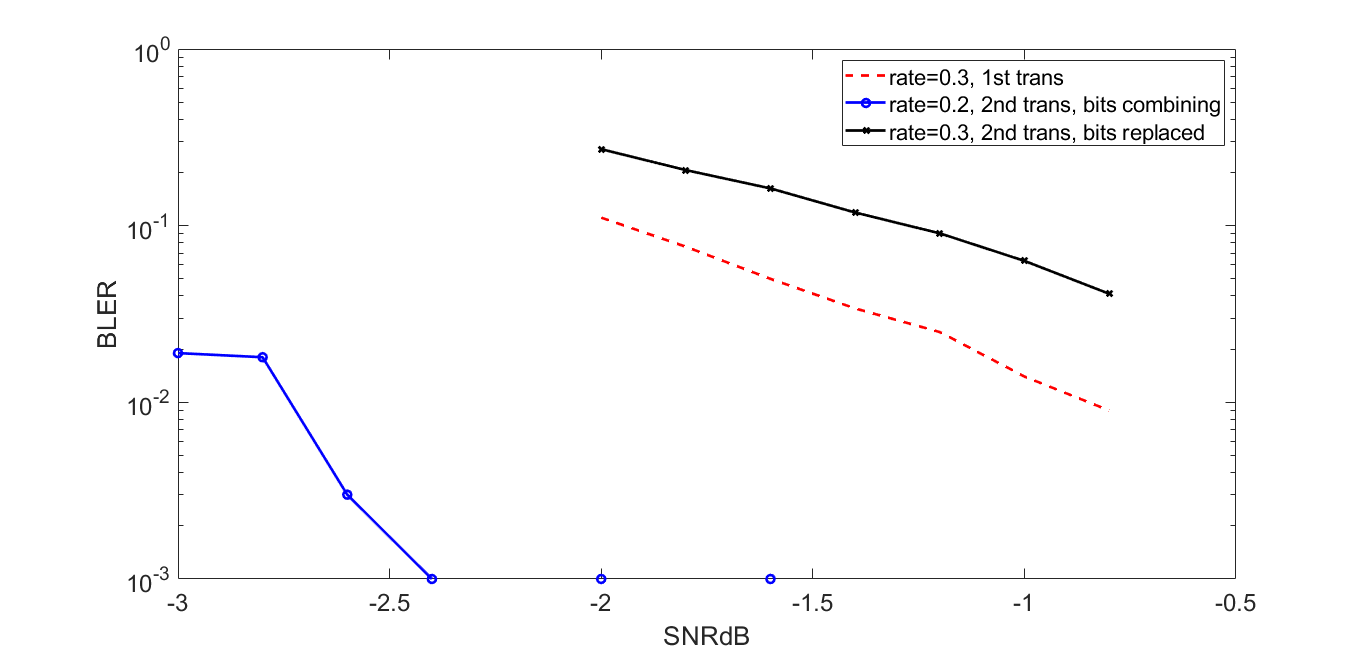
\includegraphics[scale=0.43]{fig9.png}}
\caption{BLER of the combined PDCCH in different scheme.}
\label{fig9}
\end{figure}

Fig.~\ref{fig9} shows BLER of PDCCH combined with the additional bits compared to that of PDCCH where half of bits are replaced by the bits in the better retransmission channel. The BLER of the codeword with replaced bits (black curve) is better than the first codeword (red curve) but is much worse than the codeword combined  with the additional bits (blue curve) with a margin of 2dB. Thus, in the retransmission, the additional bits due to a lower code rate should be transmitted to combine with the first codeword so the decoder works with a codeword with a lower rate and can achieve better BLER.

\section{Future work}
The abstraction of URLLC is going to be studied to build a theoretical model. After that, based on this theoretical model, the aspects of URLLC will be implemented in a simulator at system level. The more exact quantification of the proposed scheme will be done with this system simulator.

\section{Conclusion}

The emergence of URLLC in 5G requires an improvement in physical layer design. The state-of-the-art schemes achieve reliability at cost of latency and resource. In this paper, a downlink transmission scheme applying an intelligent combining based approach to get improved PDCCH and PDSCH detection while reducing latency and resource consumption is presented. The designs of PDCCH and PDSCH and the techniques to implement the combining are also explained. 

\begin{thebibliography}{00}
\bibitem{ad1} H. Ji, S. Park, J. Yeo, Y. Kim, J. Lee, and B. Shim, “Ultra Reliable and Low Latency Communications in 5G Downlink: Physical Layer Aspects,”  IEEE Wireless Commun, June 2018.
\bibitem{b9} A. Balatsoukas-Stimming, M. Bastani Parizi, and A. Burg, ``LLR-Based Successive Cancellation List Decoding of Polar Codes,'' IEEE Trans. Signal Process., vol. 63, no. 19, pp. 5165–5179, Oct 2015.
\bibitem{ad5} T-K. Le, F. Kaltenberger, U. Salim, ``Ultra-reliable and low-latency communication's downlink transmission with two-stage feedback,'' submitted to 2019 IEEE 17th Wireless Communications and Networking Conference, April 2019.
\bibitem{b1} Intel Corporation, ``Ultra-reliability for NR PDCCH'', 3GPP R1-1717381, RAN1\#90bis, Prague, Czech Republic, Oct 9--13, 2017.
\bibitem{b2} Huawei, HiSilicon, ``PDCCH reliability for URLLC'', 3GPP R1-1719406, RAN1\#91, Reno, USA, Nov 27--Dec1, 2017.
\bibitem{b3} MediaTek Inc, ``HARQ design and PDCCH reliability for URLLC'', 3GPP R1-1716620, RAN1 Ad Hoc\#3, Nagoya, Japan, Sept 18--21, 2017.
\bibitem{b4} Sony, ``Reliable PDCCH operation for NR'', 3GPP R1-1716248, RAN1 Ad Hoc\#3, Nagoya, Japan, Sept 18--21, 2017.
\bibitem{b5} Sequans Communications, ``On PDCCH repetition for NR URLLC'', 3GPP R1-1802534, RAN1\#92, Athens, Greece, Feb 26--March 2, 2018.
\bibitem{b7} ZTE, ZTE Microelectronics, ``Analysis of URLLC reliability for HARQ'', 3GPP R1-1701595, RAN1\#88, Athens, Greece, Feb 13--17, 2017.
\bibitem{ad3} 3GPP TR 38.802 v14.1.0, ``Study on new radio access technology physical layer aspects.''
\bibitem{b6} 3GPP TR 38.913 v14.3.0, ``Study on scenarios and requirements for next generation access technologies.''
\bibitem{ad2} 3GPP TR 38.211 v15.0.0, ``Physical channels and modulation.''
\bibitem{b8} 3GPP TR 38.212 v15.0.0, ``Multiplexing and channel coding.''
\bibitem{ad4} Chairman's Notes RAN1 \#90, Prague, Czech Republic, Aug 21--25, 2017.

\end{thebibliography}
\vspace{12pt}


\end{document}
